\documentclass[aspectratio=169]{beamer}
\input{../utils/beamerpreamble.tex}

\subtitle[Benchmarking Experiment Paper: Part II]{Paper Study -- "Benchmarking in Optimization: Best Practice and Open Issues"\\Part II}
\date{}

\begin{document}

\begin{frame}
  \maketitle

  \vfill

  \hfill \tiny{Version 2024.1 (Updated \today)}
\end{frame}

\section{Outline}

\begin{frame}[t]{Outline}
  We continue the study of the "Benchmarking Best Practices" paper. The topics for the second half are:\medskip
  \begin{itemize}
    \item Analyzing the results;
    \item Selecting of experimental parameters;
    \item Reporting the Results;
  \end{itemize}\bigskip

  \begin{block}{}
  https://arxiv.org/abs/2007.03488\medskip
  
  The paper focuses on the study of optimization methods, but its suggestions are highly applicable for other CS areas as well.
  \end{block}
\end{frame}

\begin{frame}[t]{Review: What is an optimization problem?}

  \begin{columns}
    \column{0.6\textwidth}
    Consider the following problem: You want to leave from your home, and reach a beautiful island. You walking speed is 8mph, and your swimming speed is 3mph.\bigskip

    What is the optimal (fastest) location for you to switch from walking to swimming?\bigskip 

    This problem can be represented as an equation, and you can find the answer by calculating the value of $x$ that minimizes $T(x)$

    \column{0.4\textwidth}
    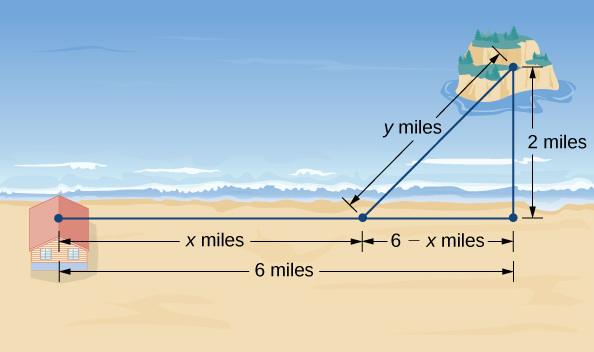
\includegraphics[width=\textwidth]{img/beach_optimization.jpeg}
    \ppagenote{Beach Optimization Image from math.libretexts.org.}
    \medskip

    Equation for the beach problem:
    \begin{equation*}
      T(x) = \frac{x}{8} + \frac{\sqrt{(6-x)^2 + 4}}{3}
    \end{equation*}
  \end{columns}
\end{frame}

\begin{frame}[t]{Optimization Benchmark Problems}
  \begin{columns}
    \column{0.6\textwidth}
    Most optimization problems are much more complicaded. Benchmark functions can replicate these conditions:\medskip

    \begin{itemize}
      \item Griewank benchmark problem (2 dimensions); 
      $G(x) = 1+\frac{1}{4000}x^2_1+\frac{1}{4000}x^2_2-\cos(x_1)\cos(\frac{1}{2}x_2\sqrt(2))$\medskip
      \item Gomez and Levy problem (modified);
      $GL(x,y) = 4x^2 - 2.1x^4 + \frac{1}{3}x^6 + xy - 4y^2 + 4y^4$\\
      subjected to: $-\sin(4\pi x)+2\sin^2(2\pi y) \leq 1.5$
    \end{itemize}\medskip

    There are large sets of benchmark problems like this, such as the CEC, BBOB, etc.

    \column{0.4\textwidth}
    \begin{center}
    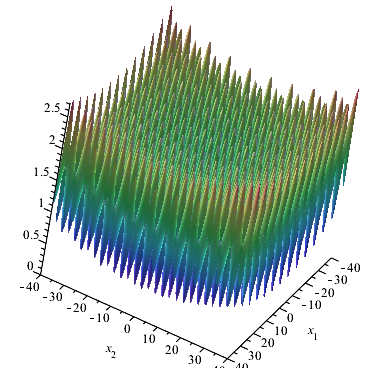
\includegraphics[width=.6\textwidth]{img/Griewank_function_3D_plot.png}
    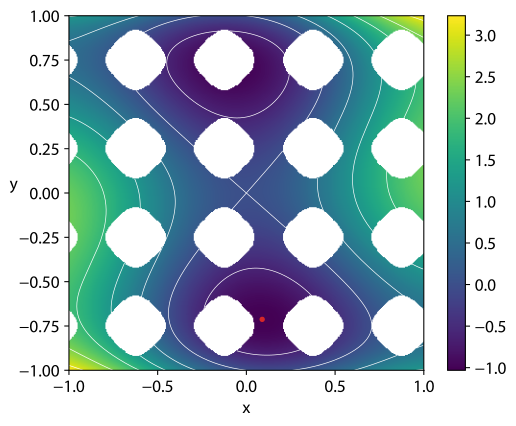
\includegraphics[width=.6\textwidth]{img/Gomez-Levi_contour.png}
    \end{center}
    \ppagenote{Griewank function by Gisling, Gomez-Levi function by Nschloe, CC BY-SA 4.0, Wikimedia foundation.}
  \end{columns}
\end{frame}


\begin{frame}[t]{Optimization Algorithms}
  Optimization algorithms try to find the value of $x$ (vector) that minimize (or maximize) the problem function.\bigskip 

  There are many different optimization algorithms, and each algorithm can be further configured with different parameters:

  \begin{itemize}
    \item Genetic Algorithm;
    \item Evolution Strategies;
    \item Particle Swarm Optimization;
    \item CMA-ES;
    \item and many others...
  \end{itemize}\bigskip

  We will focus on \structure{Metaheuristic} optimization algorithms, which work by testing several candidate values for $x$ until they find the optimum.
  
\end{frame}


\section{Analysis of the Results}

\begin{frame}[t]{Three-Level Approach for Result Analysis}
  In the first half we discussed the selection of goal, algorithms, datasets and measures for the experiment. After that, we perform the experiment and collect the data. {\bf The next step is to analyze the data and draw conclusions} from it.\medskip
  
  {\bf Consider a comparison experiment}, between one or more algorithm configurations, on one or more problem instances.\medskip 

  We can divide the analysis in a three level approach:
  \begin{itemize}
    \item Exploratory Data Analysis (EDA)
    \item Confirmatory Analysis
    \item Relevance Analysis
  \end{itemize}

  \vfill 
  Please check the many references for each of these levels in the original paper.
\end{frame}

\subsection{Exploratory Data Analysis}

\begin{frame}[t]{Exploratory Data Analysis (EDA)}
  Descriptive and graphical techniques for an initial understanding of the results:
  \begin{itemize}
    \item Verify the \structure{distribution} of the data; 
    \item Check underlying assumptions: \structure{Normality, equality of variances};
    \item \structure{Visualize basic patterns} in the data: outliers, dependencies;
    \item Catch possible bugs in the implementation;
    \item "Let the data speak"
  \end{itemize}
  \vfill 

  \begin{quote}
    Exploratory Data Analysis is based on experience, judgement and artistry: there is no standard cookbook, but many recipes.
  \end{quote}
\end{frame}

\begin{frame}[t]{EDA: The Glorious Seven}
  Standard metrics that we want to calculate from the sample: 
  \begin{itemize}
    \item Mean
    \item Median 
    \item Minimum
    \item Maximum
    \item First Quartile
    \item Third Quartile
    \item Standard Deviation
  \end{itemize}\bigskip 

  These values may be \structure{Sensitive to outliers, missing or biased data}.\medskip 

  These values are important, but they are based on that specific experiment only, so {\bf they do not provide a complete analysis of the performance}.
\end{frame}

\begin{frame}[t]{EDA: Graphical Tools -- Boxplot}
  \begin{columns}
    \column{0.6\textwidth}
    The Boxplot visualizes the {\bf Median, First Quartile, Third Quartile} of a sample, as well as the 5 and 95 percentiles.\bigskip 

    They can show the spread of a sample in a very compact way, and are also useful for visually comparing multiple samples.\bigskip

    A boxplot that includes density information is a {\bf Violin Plot}.
    \column{0.4\textwidth}
    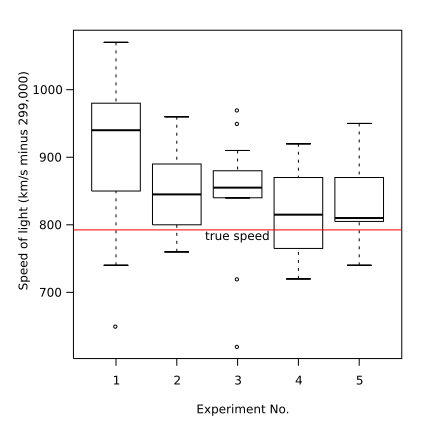
\includegraphics[width=1\textwidth]{img/Michelsonmorley-boxplot.png}
    \ppagenote{Example of Boxplot from Wikipedia -- Boxplots}
  \end{columns}
  
\end{frame}

\begin{frame}[t]{EDA: Graphical Tools -- Histogram}
  \begin{columns}
    \column{0.5\textwidth}
    The Histogram can show the shape of distribution of the data in the sample, and also give an idea of the statistical bias and spread of the data.\bigskip 

    The histogram is very sensitive to the size of the boxes (\emph{bins}), so it is suggested to combine histograms with density plots.
    \column{0.5\textwidth}
    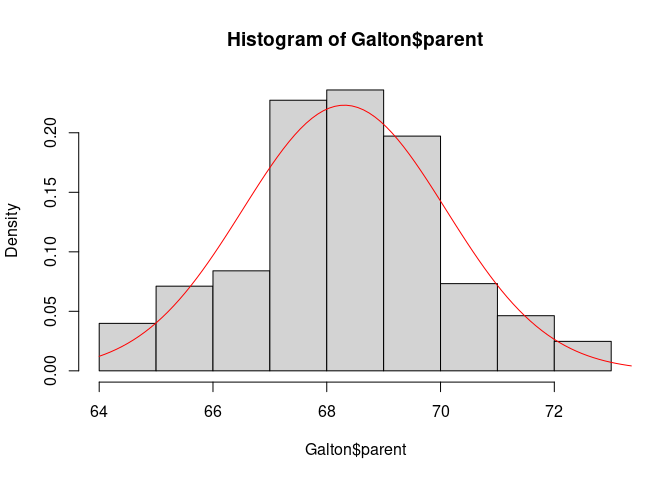
\includegraphics[width=1\textwidth]{img/Histogram_Density.png}
    \ppagenote{Example of Histogram/Density Plot from University of Iowa - STAT:4580 https://homepage.divms.uiowa.edu/~luke/classes/STAT4580/histdens.html}
  \end{columns}
  
\end{frame}

\begin{frame}[t]{EDA: Graphical Tools -- Experiment Specific Tools}
  \begin{columns}
    \column{0.6\textwidth}
    In addition to graphs that show aggregate results of the experiment, optimization research often uses specific graphs that show the behavior of algorithms in detail, such as:\bigskip

    \begin{itemize}
      \item {\bf Run-time Behavior}
      \item {\bf Performance Profiles}
      \item {\bf Data Profiles}
    \end{itemize}\bigskip

    Runtime behavior is the most commonly used for comparing metaheuristic algorithms.

    \column{0.4\textwidth}
    \begin{center}
    Run-time behavior graph example
    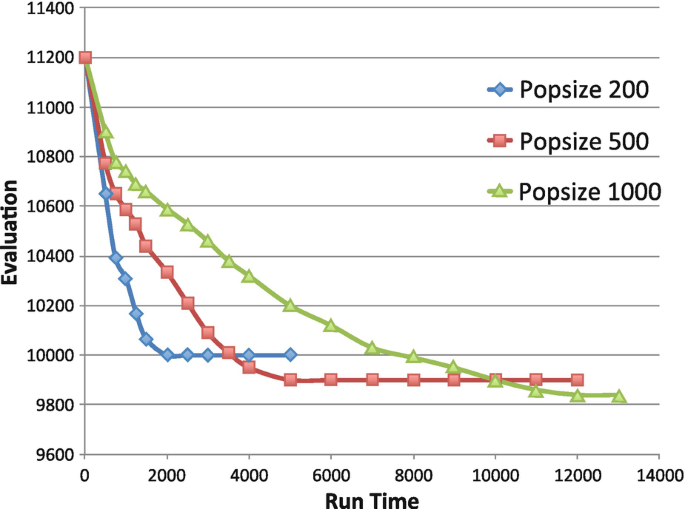
\includegraphics[width=1\textwidth]{img/runtime_springer.png}
    \end{center}
    \ppagenote{Example of Runtime Behavior graph from "Next Generation Genetic Algorithms: A User's Guide and Tutorial", by Darrel Whitley, in "Handbook of Metaheuristics", page 245--274, 2018}
  \end{columns}
\end{frame}

\subsection{Confirmatory Analysis}

\begin{frame}[t]{Confirmatory Analysis}
  After the EDA step, the Confirmatory Analysis level uses \structure{Inferential Statistical Tests} to verify differences of smaller magnitude when comparing different algorithm configurations.\bigskip 

  In this stage, the characteristics of the experiment should be analyzed to choose the most appropriate statistical test: 
  \begin{itemize}
    \item Number of data samples;
    \item Conditions for using parametric tests;\\
    \hfill(independence, normality, homoscedasticity of variances)
    \item Verification if the data is paired or unpaired;
  \end{itemize}\bigskip 

  The choice and procedure of the test follow the ideas already described earlier in this course.
\end{frame}

\begin{frame}{Confirmatory Analysis -- Pipeline for selecting statistical tests}
  \begin{center}
    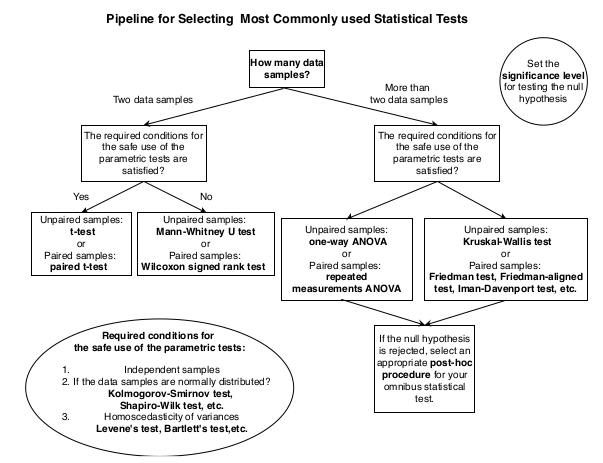
\includegraphics[width=.55\textwidth]{img/pipeline_tests.png}
  \end{center}
  \ppagenote{Pipeline for selecting statistical tests from Eftimov et al. 2020 -- check Benchmark paper for full reference}
\end{frame}

\subsection{Relevance Analysis}

\begin{frame}[t]{Relevance Analysis}
  After the statistical confirmatory analysis, the third step is to validate these results: "Are the differences meaninguful in practice or only statistical artifacts"?\bigskip 

  \begin{exampleblock}{Assembly line}
    Two optimization algorithms to minimize the time of a production process are compared. The mean difference in performance is $\delta = 10^{-14}$ which is statistically relevant. However, this difference has no meaning in reality, because it is below the precision of the timer.
  \end{exampleblock}\bigskip 

  The performance measures in benchmark studies can be affected by factors that are irrelevant in the final application, such as: computer accuracy (floating point), variable types, and stopping criteria.
\end{frame}

\begin{frame}{Relevance Analysis: Severity Measure}
  Severity is a measure that can be used to determine the meaningfulness of a statistically significant result.\bigskip 

  Severity is calculated as the power of a post-hoc data analysis that evaluates how well the data fits the testing framework of the original hypothesis.\bigskip 

  The calculation of the severity measure deals directly with the \structure{problem of large n} that can happen in simulated benchmarking experiments.
\end{frame}

\begin{frame}{Relevance Analysis: Multiple-Problem Analysis}
  When comparing the results over multiple problems (benchmark sets), it is very important to define a \structure{draw threshold}: A value where even statistically significant differences are considered to be equal from an algorithm comparison point of view.\bigskip

  Using the draw threshold, recent techniques have been developed to evaluate the practical relevance of a comparison, such as "Chess Rating Systems" and "practical Deep Statistical Comparison".\bigskip 

  In practice, there are still several open questions regarding the evaluation of problem relevance in benchmark studies.
\end{frame}

\section{Experimental Design}

\begin{frame}{Experimental Design}
  In experiments comparing algorithm configurations, "experimental design" usually refers to how we choose the parameters of the configurations that we want to compare. Some key concepts:\bigskip 

  \begin{itemize}
    \item \structure{Design Space}: The combination of all variables under consideration;
    \item \structure{Sequential design}: The choice of parameters happens after each result is investigated;
    \item \structure{One Factor At a Time}: Sequential design where each parameter is investigated in order, fixing all the others;
    \item \structure{Factorial design}: All combinations of parameters are investigated;
    \item \structure{Space filling design}: A representative set of parameters are investigated; (example: Latin Hypercube)
  \end{itemize}
  
  Selection of the design depends on the goals and characteristics of the experiment.
\end{frame}

\section{Presentation of Results}

\begin{frame}{Presentation of Results}{Recommendations from Gent and Walsh (1994)}
  General ideas for improving the production of the paper with the experiment Results.\bigskip 

  \begin{itemize}
    \item Present statistics when describing the comparison between two algorithms; 
    \item Do not push deadlines: Plan your experiment, analisis and writing to have enough time to carefully analyse the results. Spend time planning the Exploratory Analysis as well.
    \item Report Negative results: Present and discuss problem instances where the algorithm performs badly or does not perform as expected (key component of a scientific report as opposed to a PR piece)
  \end{itemize}

  The section lists several other papers with good advice and principles for scientific reporting.
\end{frame}

\begin{frame}{Considerations about Reproducibility: Levels of Reproducibility}
  \begin{itemize}
    \item {\bf Repeatability}: Same team, same experimental setup.\bigskip 
    \item {\bf Reproducibility}: Different team, different experimental setup.\bigskip
    \item {\bf Replicability}: Different team, different experimental setup.
  \end{itemize}
\end{frame}

\section{Summary}

\begin{frame}[t]{Final Considerations}
  \begin{itemize}
    \item Read the paper for more details and further discussion;
    \item Example exam in manaba; 
    \item Files for Report 2 are delayed. I hope they will be finished this weekend.
    \item I will change the grade to: $R_1*0.4 + \text{max}(R_2, E)*0.6$
  \end{itemize}
\end{frame}

%%%%%%%%%%%%%%%%%%%%%%%%%%%%%%%%%%%%%%%%%%%%%%%%%%%%
\input{../utils/lastslide.tex}
\end{document}